\documentclass[11pt, a4papper]{report}
\usepackage{amsthm}
\usepackage{amssymb, amsmath}
\usepackage{array}
\usepackage[romanian]{babel}
\usepackage{bm}
\usepackage{enumerate}
\usepackage{float}
\usepackage{geometry}
\usepackage{graphicx}
\usepackage{listings}
\usepackage{longtable}
\usepackage[utf8]{inputenc}
\usepackage{listings}
\usepackage{colortbl}
\usepackage[svgnames]{xcolor}
\usepackage{bbding}
\usepackage{pifont}
\usepackage{wasysym}
\usepackage{subcaption}
\DeclareMathOperator*{\minimize}{argmin}
\DeclareMathOperator*{\limi}{lim}
\usepackage[linesnumbered,ruled,vlined]{algorithm2e}
\usepackage{algpseudocode}

\newcommand\mycommfont[1]{\footnotesize\ttfamily\textcolor{blue}{#1}}
\SetCommentSty{mycommfont}

\SetKwInput{KwInput}{Input}                
\SetKwInput{KwOutput}{Output}              

\theoremstyle{plain}
\newtheorem{theorem}{Theorem}

\theoremstyle{definition}
\newtheorem{definition}{Definition}

\theoremstyle{definition}
\newtheorem{lemma}{Lemma}

\newcolumntype{M}[1]{>{\centering\arraybackslash}m{#1}}

\lstset{language=R,
    basicstyle=\small\ttfamily,
    stringstyle=\color{DarkGreen},
    otherkeywords={0,1,2,3,4,5,6,7,8,9},
    morekeywords={TRUE,FALSE},
    deletekeywords={data,frame,length,as,character},
    keywordstyle=\color{blue},
    commentstyle=\color{DarkGreen},
}


\theoremstyle{proposition}
\newtheorem{proposition}{Proposition}

 \geometry{
 a4paper,
 total={160mm,257mm},
 left=30mm,
 right=20mm,
 top=20mm,
 bottom=20mm,
 }
 
\setcounter{tocdepth}{4}
\setcounter{secnumdepth}{4}
\renewcommand{\baselinestretch}{1.25}
 
\graphicspath{ {Images/} }

 

\addto\captionsromanian{% Replace "english" with the language you use
  \renewcommand{\contentsname}%
    {Contents}%
}

\begin{document}
\begin{center}

\vspace*{.06\textheight}
{\scshape\large {``Alexandru Ioan Cuza" University of Iaşi}\par}\vspace{0.3cm} 
\textsc{\large {Master of computational optimization}}\\[0.3cm] 
\textbf{\textsc{\large {FACULTY OF COMPUTER SCIENCE }}}\\[1.3cm] 


\vspace{0.4cm}
\textsc{\large {Advanced Software Engineering Techniques 2019 Project}}\\[0.1cm]
\textsc{\large { - State of the art - }}\\[2.7cm]

\vspace{0.6cm}
{\LARGE \bfseries {Freesound Audio Tagging 2019}\par}
\vspace{0.2cm} 
{\Large \bfseries {Automatically recognize sounds and apply tags of varying natures}\par}


\vspace{4.4cm}

\begin{center}
\textsc{\large Proposed by: Cojocaru Gabriel-Codrin}\\
\textsc{\large Dinu Sergiu Andrei} \\
\textsc{\large Luncașu Bogdan Cristian} \\
\textsc{\large Racoviță Mădălina-Alina} \\
\textsc{\large Vîntur Cristian} \\
[3.1cm]
\textsc{\large Scientific coordinators}: {\textsc{\large PhD Associate Professor Adrian Iftene}} \\
{\textsc{\large PhD Associate Professor Mihaela Elena Breaban}}
\end{center}
\end{center}
\newpage

%----------------------------------------------------------------------------------------
%	Table of contents
%----------------------------------------------------------------------------------------

\addcontentsline{toc}{chapter}{Contents}

\tableofcontents

\newpage

%----------------------------------------------------------------------------------------
%	The environmental sound classification problem
%----------------------------------------------------------------------------------------

\addcontentsline{toc}{chapter}{State of the art}
\chapter*{State of the art}

\addcontentsline{toc}{section}{Problem description}
\section*{Problem description}

The environmental sound classification problem can come in many different shapes, from having to classify short audio files with a label from a specified set to having to tag live audio streaming with one or multiple labels.
\\

Automatic environmental sound classification or tagging is a growing area of research. Work done in this area is comparatively scarce with work done in related audio fields such as speech and music. Applications are numerous and include multimedia indexing and retrieval, environmental sounds subtitles, assisting deaf individuals or even monitoring illegal deforestation. A very interesting project regarding this last use case is created by a non-profit organization called Delta Analytics. They helped build a system where a lot of old mobile phones are attached to trees in rain forests which listen to chainsaw noises. Their role is to identify when a chainsaw is being used and alert rangers who can stop illegal deforestation.
\\

Because of the recent success in image classification, the question that raises is: can we bring techniques used in image classification to sound classification by representing sound in various image formats?

\addcontentsline{toc}{section}{Short audio files classification}
\section*{Short audio files classification}

\addcontentsline{toc}{subsection}{Problem statement}
\subsection*{Problem statement}

Classify environmental sounds with focus on identification of particular urban sounds. Given an audio sample of a few seconds duration determine if it contains one of the target urban sounds.

\addcontentsline{toc}{subsection}{Dataset description}
\subsection*{Dataset description}

The dataset is called Urbansound8K and contains 8732 sound excerpts (under 4s) of urban sounds from 10 classes, which are:

\begin{itemize}
\item Air Conditioner
\item Car Horn
\item Children Playing
\item Dog bark
\item Drilling
\item Engine Idling
\item Gun Shot
\item Jackhammer
\item Siren
\item Street Music
\end{itemize}

By taking a closer look to the dataset, the following observation can be made: it's tricky to visualize the difference between some sounds, especially the continuous ones like jackhammer and engine idling.

\begin{center}
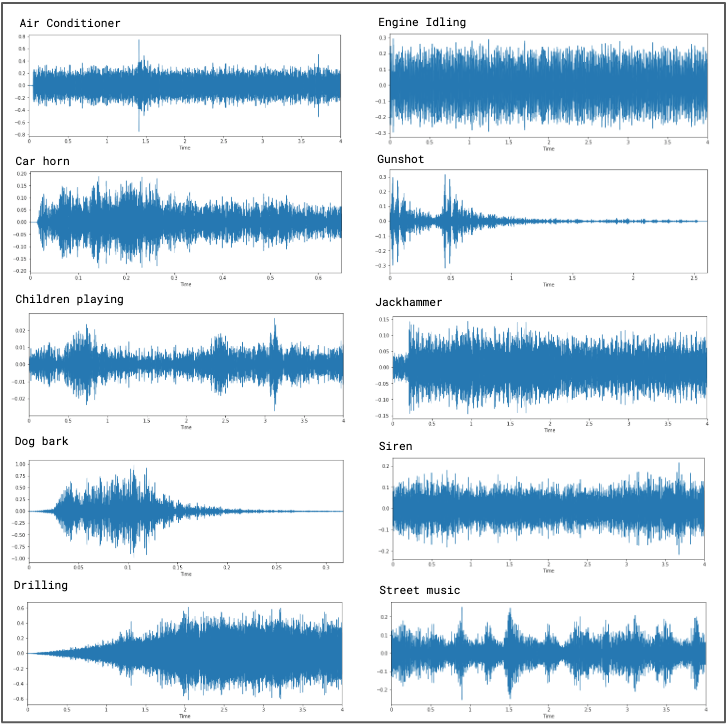
\includegraphics[scale=0.6]{sound-waves.png}
\end{center}
\begin{center}
\textbf{Fig. }: \textit{Visualization of sound amplitude with respect to time}
\end{center}

A deeper dive into the data show that: most samples have 2 audio channels with a few having just 1 channel, sample rate varies from 8kHz to 48kHZ and bit depth also varies from 4bit to 32bit which leads to requiring a data normalization step.

\addcontentsline{toc}{subsection}{Proposed solution}
\subsection*{Proposed solution}
The proposed solution involves mapping the audio files, after the normalization step, to a visual representation. Spectrograms are a useful technique for visualizing the spectrum of frequencies of a sound and how they vary during a very short period of time. A similar technique known as mel-spectrogram will be used for this case. The main difference is that a spectrogram uses a linear spaced frequency scale (so each frequency bin is spaced an equal number of Hertz apart), whereas a mel-spectrogram uses a quasi-logarithmic spaced frequency scale, which is more similar to how the human auditory system processes sounds.

\begin{center}
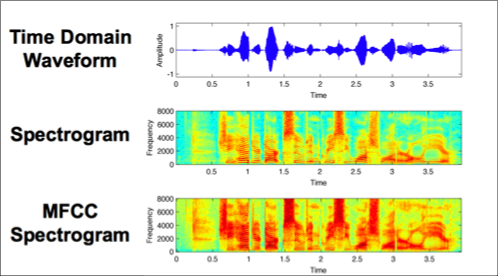
\includegraphics[scale=0.8]{sound-representation.png}
\end{center}
\begin{center}
\textbf{Fig. }: \textit{Spectrogram and mel-spectrogram}
\end{center}

The problem will be solved by using deep learning on the visual representation of the audio file. In this case a Convolutional Neural Network (CNN) will be used. The model used is a sequantial one consisting of 4 Conv2D convolution layers with the final output being a dense layer. The output layer will have 10 nodes which matches the number of possible classifications.

\addcontentsline{toc}{subsection}{Results}
\subsection*{Results}
The trained model obtained a Training accuracy of 98.19\% and a Testing accuracy of 91.92\%.

\addcontentsline{toc}{section}{Tagging longer audio files}
\section*{Tagging longer audio files}

By providing a solution to solving the short audio files tagging problem we can extend it to work on longer audio files. The idea behind this extension is to divide the audio into smaller parts, transform these parts into mel-spectrograms and feed them into a more complex network that will be able to provide the correct label(s).

\addcontentsline{toc}{section}{State of the art}
\section*{State of the art solution}
State of the art solution to solving this problem is deep learning. By dividing the audio and transforming it into mel-spectrograms we can use some of the success of image classification and bring it to audio classification. Just applying image classification on mel-spectrograms doesn't work because sound in form of mel-spectrograms doesn't have the same properties as an image but by adapting the network the the new context we can obtain a solution to solving this problem.

\addcontentsline{toc}{section}{Relevant articles}
\section*{Relevant articles}

\begin{itemize}
\item AUDIO TAGGING WITH NOISY LABELS AND MINIMAL SUPERVISION - \\ \textit{https://arxiv.org/pdf/1906.02975.pdf}
\item Convolutional RNN: an Enhanced Model for
Extracting Features from Sequential Data - \textit{https://arxiv.org/pdf/1602.05875v3.pdf}
\end{itemize}

\addcontentsline{toc}{section}{Relevant articles}
\section*{Relevant links}

\begin{itemize}
\item Kaggle competition 1st place solution - \textit{https://github.com/lRomul/argus-freesound}
\item Kaggle competition 2nd place solution - \textit{https://www.kaggle.com/c/freesound-audio-tagging-2019/discussion/97815}
\item Kaggle competition 3rd place solution - \textit{https://www.kaggle.com/c/freesound-audio-tagging-2019/discussion/97926}
\end{itemize}

%----------------------------------------------------------------------------------------
%	Bibliography
%----------------------------------------------------------------------------------------

\addcontentsline{toc}{chapter}{Bibliography}
\bibliographystyle{unsrt}

\begin{thebibliography}{1}

\bibitem[]{} \textbf{"Classifying Urban sounds using Deep Learning"}, Mike Smales: \textit{https://github.com/mikesmales/Udacity-ML-Capstone/blob/master/Report/Report.pdf}

\bibitem[]{} \textbf{"Data Science for Good: Stopping Illegal Deforestat"}, Sara Hooker, Sean McPherson: \textit{https://mlconf.com/sessions/data-science-for-good-stopping-illegal-deforestat-2/}

\bibitem[]{} Eduardo Fonseca, Manoj Plakal, Frederic Font, Daniel P. W. Ellis, Xavier Serra.\\ \textbf{"AUDIO TAGGING WITH NOISY LABELS AND MINIMAL SUPERVISION"} in Detection and Classification of Acoustic Scenes and Events 2019 [PDF]

\end{thebibliography}

\end{document}